\chapter{实时操作系统VxWorks}

\section{概述}

\subsection{实时操作系统}
实时操作系统(Real Time Operation System,简称RTOS)是整个实时系统的核心。POSIX1003.1标准为RTOS下了一个简单的定义:RTOS是能够在有限的响应时间内为应用提供所要求级别服务的操作系统\cite{Renard20081003}。当外界事件或者是数据产生时,RTOS需要快速的进行处理,并且处理的结果又能够在规定的时间之内来控制生产过程或者对处理系统做出快速的响应,调度一切可利用的资源来完成实时任务。实时系统按照实时的效果可以分为软实时和硬实时,硬实时要求在规定的时间内必须完成操作,这是通过操作的在设计的时候就得到保证的;软实时只需要按照任务的优先级,尽可能快的完成任务即可。

一个实时操作系统的特征通常包括以下几点:
\begin{itemize}
\item \textbf{高精度计时系统} 

计时精度是影响实时性的一个重要因素,在实时系统当中,经常需要精确确定实时地操作某个设备或执行某个任务,或精确的计算一个时间函数。这些不仅仅依赖于一些硬件提供的时钟精度,也依赖于实时操作系统的高精度计时功能。
\item \textbf{多级中断机制}

中断是实时操作系统当中的一个关键设施,是用于通知系统发生外部事件的常用机制。一个实时操作系统通常需要处理多种外部信息或事件,但处理的紧迫程度有轻重缓急之分。有的必须立即作出反应,有的则可以延后处理。因此,需要建立多级中断嵌套处理机制,以确保对紧迫程度较高的实时事件进行及时响应和处理。
\item \textbf{实时调度机制} 

实时操作系统不仅要及时响应实时事件中断,同时也要及时调度运行实时任务。但是,处理机调度并不能随心所欲的进行,因为涉及到两个进程之间的切换,只能在确保“安全切换”的时间点上进行,实时调度机制包括两个方面,一是在调度策略和算法上保证优先调度实时任务;二是建立更多“安全切换”时间点,保证及时调度实时任务。
\end{itemize}

	内核作为操作系统的核心,负责控制这计算机上的所有硬件和软件资源,在必要的时候给应用程序分配硬件资源,并执行相应的操作命令。内核的主要功能为以下四个:
\begin{itemize}
\item 系统内存管理
\item 软件程序管理
\item 硬件设备管理
\item 文件和网络系统管理
\end{itemize}

本次所需完成的调试通道正是基于一个目前业界有名的实时操作系统VxWorks。

\subsection{VxWorks简介}
	VxWorks操作系统是美国Wind River System公司于1983年推出的一个运行在目标机上的高性能、可裁剪的实时操作系统(RTOS),该系统专门为嵌入式实时系统领域而设计开发,其具有良好的持续发展能力、高性能的内核以及友好的用户开发环境,为开发人员提供了高效的实时多任务调度、中断管理、实时的系统资源以及实时的任务间通信。并且拥有多达1800个功能强大的应用程序接口\cite{嵌入式实时操作系统VxWorks及其开发环境Tornado}。
	
	VxWorks采用微内核设计,支持多种硬件环境,包括X86、PowerPC、ARM等众多主流的处理器,同时还支持RISC、DSP技术,且在各种CPU平台上提供了统一的编程接口和一致的运行环境。VxWorks凭借着其优异的性能在军事、航空航天、工业控制、通信等高精尖以及实时性要求极高的领域当中,有着更加广泛而深入的应用。应用实例包括火星探测器、爱国者导弹、飞机导航、F-16、FA-18战斗机等\cite{嵌入式实时操作系统VxWorks及其开发环境Tornado}。自从对我国的销售解禁之后,VxWorks也大量的应用于我国的军事、国防工业当中。
	
	VxWorks操作系统由400多个相对独立的短小精炼的目标模块组成,用户可以根据自己的实际需求选择适当的模板来裁剪和配置系统,这样可以有效的保证系统的安全性和可靠性。系统的连接器可以按照应用的需要自动链接一些目标模块。这样,通过目标模块之间的按需组合,可以得到许多满足功能需求的应用。此外,VxWorks支持广泛的工业标准,如POSIX1003.1b实时扩展、ANSIC(浮点支持)和TCP/IP网络协议等。这种广泛的协议支持在主机和目标机之间提供了无缝的工作环境,任务可以通过网络箱其他系统的主机存取文件,即远程文件存取,也支持远程的过程调用。这些标准也促进了多种不同产品之间的互通性,提升了可移植性。由于其高度的灵活性,用户能够很容易的对该操作系统进行重新定制或作适当的开发,以满足自己的实际应用。

\section{微内核wind}

\subsection{wind的多任务机制}
现代实时系统基于多任务和任务间通信的互补概念。多任务环境允许将实时应用程序构建为一组独立任务,每个任务都有自己的执行线程和一组系统资源。任务间通信设施允许这些任务同步并进行通信以协调其活动。在VxWorks中,任务间的通信工具包括快速信号量、消息队列、管道、套接字。


\subsection{wind的任务调度}

\subsection{wind线程同步}

\section{集成开发环境Tornado}
\subsection{tadj}

\section{VxWorsks上的USB协议栈}
	USB(Universial Serial Bus,通用串行总线)是这十几年来应用在PC领域的最新型的接口技术,出现的契机是为了为了解决日益增加的PC外设与有限的主板插槽之间的矛盾,其实现的原理是由一些PC大厂商(Microsoft、Intel等)定制出来的,自从1995年在Comdex上展出以来至今已广泛地被各个PC厂家所支持。目前已经在各类外部设备中都广泛的采用USB接口。USB接口标准目前有三种:USB1.1,USB2.0和USB3.0。USB接口应用如此的广泛是由其独特和实用的特性决定的。USB的体系结构如图\autoref{fig:USB体系结构}所示
\begin{figure}[!h]
\centering
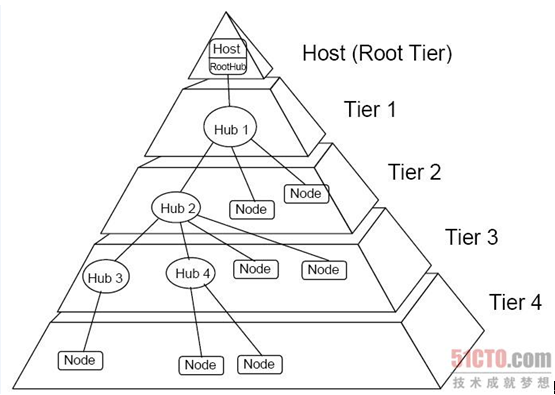
\includegraphics[width=.4\textwidth]{USB-structure.png}
\caption{USB-structure}\label{fig:USB体系结构}
\end{figure}
	

\subsection{USB数据传输的优势}
	USB的主要有优点有:
	\begin{enumerate}
	\item 使用方便,支持热插拔:连接外设不必再打开主机箱,而且方便携带,允许在任何时候USB外设的热插拔,而且不必关闭主机的电源;USB外设没有需要用户选择的设置;例如端口地址和中断请求线;自动配置外设,当用户连接USB外设到一个正在运行的系统时,系统会自动的检测外设,载入合适的驱动软件(如果有的话),并将其初始化;以上的特点使得USB外设符合便携易用的潮流。
	\item 速度快:目前设备上使用大多数是USB 2.0的接口,最新生产的设备都配备了USB3.0的接口。USB2.0接口的理论速度可以达到480Mbps(即60MB/s),并且可以向下兼容USB1.1。USB3.0接口的理论速度可以达到5.0Gbps(即640MB/s),并提供USB2.0的兼容。
	\item 连接灵活:一个USB主控制器理论上可以连接127个设备
	\end{enumerate}


\subsection{VxWorks上的USB驱动程序结构}

\section{CP2012模块}
\subsection{CP2102简介}

cp2102的电路框图如\autoref{fig:cp2102电路框图}所示.

\begin{figure}[!h]
\centering
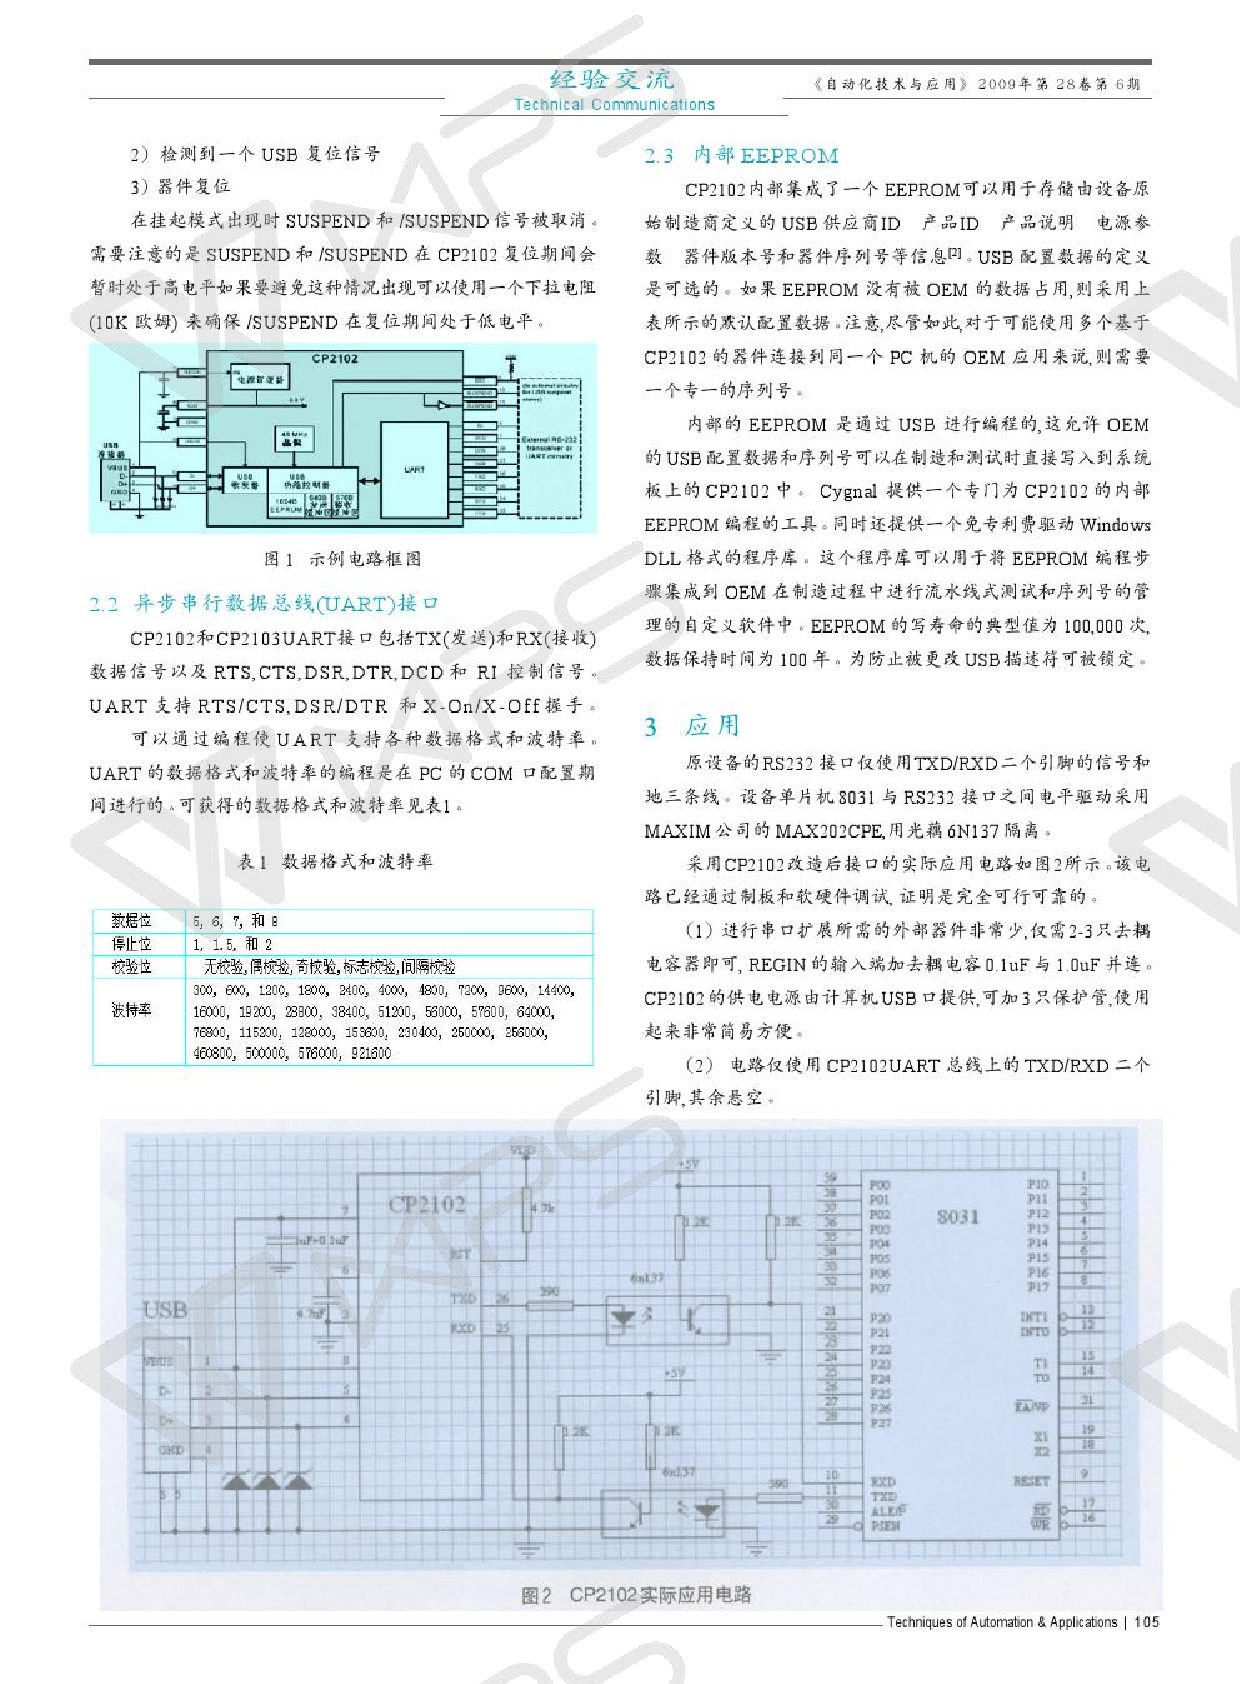
\includegraphics[width=.4\textwidth]{./graphics/cp2102-circuit-diagram.pdf}
\caption{cp2102电路框图}\label{fig:cp2102电路框图}
\end{figure}



